%!TEX root = ../dokumentation.tex

\chapter{Konzept}

Als Grundlage der Schnittstelle soll eine MATLAB-Standalone-Applikation dienen, welche eine zentrale Benutzeroberfläche für die Funktionalitäten der Anforderungen stellt. Ein Nutzer soll so in der Lage sein diese Applikation auf seinem Rechner zu starten und von hier aus eine Auswahl über die einzelnen Funktionen der Applikation zu bekommen. Der grundlegenden Benutzung der Applikation soll wie folgt stattfinden. Der Benutzer kann entweder Samples für eine Messung konfigurieren und diese dann im nächsten Schritt innerhalb des Tools visualisieren oder, bei bereits angelegten Samples, diese direkt im Graphen anzeigen. So kann die Erstellung neuer Visualisierungsdaten, aber auch die Wiederverwendbarkeit bereits angelegter Daten gewährleistet werden. Innerhalb eines Ablaufdiagramms lässt sich dies folgendermaßen beschreiben:

\begin{figure}[!htbp]
	\centering
	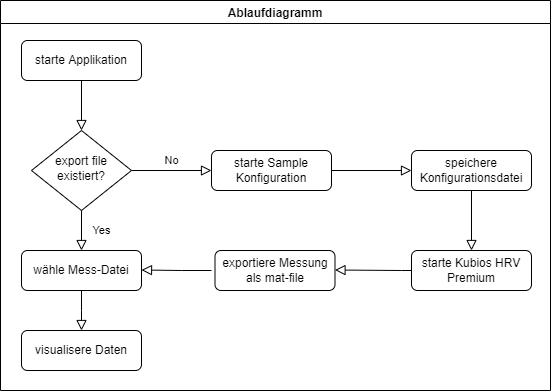
\includegraphics[width=0.8\linewidth]{ablaufKonzept}
	\caption{Ablaufdiagramm des Konzepts}
	\label{fig:ablaufKonzept}
\end{figure}

Dabei ergeben sich zwei große Bereiche in die die Applikation aufgeteilt wird und die beiden Hauptfunktionalitäten der Anforderung, das erstellen geeigneter Samples in Kubios HRV Premium und das grafische Darstellen der erzeugten medizinischen Messdaten, repräsentieren. Diese beiden Hauptfunktionalitäten sollen dazu voneinander abgekapselt dargestellt werden, wobei das Visualisieren die Basis der Applikation darstellt und die Konfiguration der Samples auf dieser aufbaut.

% vorläufiges Klassendiagramm
% Design-Konzept hinzufügen